\chapter{Specifikacija programske potpore}
		
	\section{Funkcionalni zahtjevi}
			
			\textbf{\textit{dio 1. revizije}}\\
			
			\textit{Navesti \textbf{dionike} koji imaju \textbf{interes u ovom sustavu} ili  \textbf{su nositelji odgovornosti}. To su prije svega korisnici, ali i administratori sustava, naručitelji, razvojni tim.}\\
				
			\textit{Navesti \textbf{aktore} koji izravno \textbf{koriste} ili \textbf{komuniciraju sa sustavom}. Oni mogu imati inicijatorsku ulogu, tj. započinju određene procese u sustavu ili samo sudioničku ulogu, tj. obavljaju određeni posao. Za svakog aktora navesti funkcionalne zahtjeve koji se na njega odnose.}\\
			
			
			\noindent \textbf{Dionici:}
			
			\begin{packed_enum}
				
				\item Zaposlenik
				\item Revizor
				\item Računovođa
				\item Direktor
				\item Razvojni tim
				
			\end{packed_enum}
			

			\noindent \textbf{Aktori i njihovi funkcionalni zahtjevi:}
			
			\begin{packed_enum}
				\item  \underbar{Svaki neregistrirani/neprijavljeni korisnik (inicijator) može:}

				\begin{packed_enum}
					
					\item prijaviti se u sustav
					
				\end{packed_enum}
			
				\item  \underbar{Svaki registrirani/prijavljeni korisnik (inicijator) može:}
				
				\begin{packed_enum}
					
					\item promijeniti lozinku korisničkog računa
					\item vidjeti povijest svojih skeniranja dokumenata
					\item skenirati novi dokument i:

						\begin{packed_enum}
							
							\item potvrditi točnost skeniranog dokumenta
							\item odbiti skenirani dokument

						\end{packed_enum}

				\end{packed_enum}

				\item  \underbar{Zaposlenik (inicijator) može:}
				
				\begin{packed_enum}
					
					\item poslati skenirani dokument revizoru
					
				\end{packed_enum}

				\item  \underbar{Revizor (inicijator) može:}
				
				\begin{packed_enum}
					
					\item provjeriti pristigle dokumente, uključujući svoje, i:

						\begin{packed_enum}
							
							\item potvrditi dokument i proslijediti ga nadležnom računovođi
							\item odbiti dokument

						\end{packed_enum}
					
				\end{packed_enum}

				\item  \underbar{Računovođa (inicijator) može:}

				\begin{packed_enum}
					
					\item arhivirati pristigle dokumente
					\item proslijediti pristigli dokument direktoru na potpis
					
				\end{packed_enum}

				\item  \underbar{Direktor (inicijator) može:}

				\begin{packed_enum}
					
					\item potpisati dokumente pristigle iz računovodstva
					\item vidjeti povijest svih dokumenata
					\item vidjeti povijest i statistike svih zaposlenika
					\item objaviti određeni dokument na društvene mreže 
					\item registrirati novog korisnika i dodijeliti mu ulogu
					\item obrisati postojećeg korisnika
					
				\end{packed_enum}

				\item  \underbar{Baza podataka (sudionik):}

				\begin{packed_enum}

					\item pohranjuje sve podatke o korisnicima i njihovim ovlastima
					\item pohranjuje sve podatke o skeniranim dokumentima
					
				\end{packed_enum}			

			\end{packed_enum}
	
			\eject{}
			
			\subsection{Obrasci uporabe}
				
				\subsubsection{}

					\noindent \underbar{\textbf{UC1 — Prijava u sustav}}
					\begin{packed_item}
	
						\item \textbf{Glavni sudionik:} Bilo koji korisnik
						\item  \textbf{Cilj:} Dobiti pristup korisničkom sučelju
						\item  \textbf{Sudionici:} Baza podataka
						\item  \textbf{Preduvjet:} Posjedovanje vlastitog korisničkog računa
						\item  \textbf{Opis osnovnog tijeka:}
						
						\item[] \begin{packed_enum}
	
							\item Korisnik unosi korisničko ime i lozinku
							\item Baza podataka provjerava ispravnost unesenih podataka
							\item Korisnik dobiva pristup korisničkom sučelju

						\end{packed_enum}
						
						\item  \textbf{Opis mogućih odstupanja:}
						
						\item[] \begin{packed_item}
	
							\item[2.a] Korisnik je unio neispravno korisničko ime ili lozinku
							\item[] \begin{packed_enum}
								
								\item Sustav obavještava korisnika o neuspjeloj prijavi i vraća ga na stranicu za prijavu
								
							\end{packed_enum}
							
						\end{packed_item}

					\end{packed_item}


					\noindent \underbar{\textbf{UC2 — Promjena lozinke korisničkog računa}}
					\begin{packed_item}
	
						\item \textbf{Glavni sudionik:} Bilo koji korisnik
						\item  \textbf{Cilj:} Promijeniti lozinku korisničkog računa
						\item  \textbf{Sudionici:} Baza podataka
						\item  \textbf{Preduvjet:} Korisnik je prijavljen u sustav
						\item  \textbf{Opis osnovnog tijeka:}
						
						\item[] \begin{packed_enum}
	
							\item Korisnik odabire opciju promjene lozinke računa
							\item Korisnik unosi trenutnu lozinku računa
							\item Baza podataka provjerava ispravnost unesene lozinke
							\item Korisnik unosi novu lozinku računa
							\item Baza podataka pohranjuje promjenu lozinke

						\end{packed_enum}
						
						\item  \textbf{Opis mogućih odstupanja:}
						
						\item[] \begin{packed_item}
	
							\item[3.a] Korisnik je unio neispravnu trenutnu	lozinku
							\item[] \begin{packed_enum}
								
								\item Sustav obavještava korisnika o pogrešnom unosu trenutne lozinke i vraća ga na stranicu za unos lozinke
								
							\end{packed_enum}
							
						\end{packed_item}

					\end{packed_item}


					\noindent \underbar{\textbf{UC3 — Pregled povijesti skeniranih dokumenata}}
					\begin{packed_item}
	
						\item \textbf{Glavni sudionik:} Bilo koji korisnik
						\item  \textbf{Cilj:} Vidjeti povijest svojih skeniranih dokumenata
						\item  \textbf{Sudionici:} Baza podataka
						\item  \textbf{Preduvjet:} Korisnik je prijavljen u sustav
						\item  \textbf{Opis osnovnog tijeka:}
						
						\item[] \begin{packed_enum}
	
							\item Aplikacija korisniku na početnom zaslonu prikazuje njegovu povijest skeniranih dokumenata

						\end{packed_enum}

					\end{packed_item}


					\noindent \underbar{\textbf{UC4 — Skeniranje novog dokumenta}}
					\begin{packed_item}
	
						\item \textbf{Glavni sudionik:} Bilo koji korisnik
						\item  \textbf{Cilj:} Skenirati novi dokument
						\item  \textbf{Sudionici:} Baza podataka
						\item  \textbf{Preduvjet:} Korisnik je prijavljen u sustav
						\item  \textbf{Opis osnovnog tijeka:}
						
						\item[] \begin{packed_enum}
	
							\item Korisnik na početnom zaslonu odabire opciju za skeniranje novog dokumenta
							\item Korisnik učitava dokument u obliku slike u aplikaciju
							\item Aplikacija provjerava ispravnost učitanog dokumenta
							\item Aplikacija korisniku prikazuje učitani dokument i razvsrtava ga u jednu od kategorija:

								\begin{packed_enum}
									
									\item račun
									\item ponuda
									\item interni dokument

								\end{packed_enum}

							\item Korisnik potvrđuje točnost učitanog dokumenta ili ga odbija

						\end{packed_enum}

						\item  \textbf{Opis mogućih odstupanja:}
						
						\item[] \begin{packed_item}
	
							\item[3.a] Dokument nije ispravno skeniran
							\item[] \begin{packed_enum}
								
								\item Aplikacija obavještava korisnika o neuspjelom skeniranju i vraća ga na zaslon za učitavanje dokumenta
								
							\end{packed_enum}
							
						\end{packed_item}

					\end{packed_item}


					\noindent \underbar{\textbf{UC5 — Slanje skeniranog dokumenta revizoru}}
					\begin{packed_item}
	
						\item \textbf{Glavni sudionik:} Zaposlenik
						\item  \textbf{Cilj:} Poslati skenirani dokument revizoru
						\item  \textbf{Sudionici:} Baza podataka, revizor
						\item  \textbf{Preduvjet:} Zaposlenik se prijavio u sustav skenirao je dokument
						\item  \textbf{Opis osnovnog tijeka:}
						
						\item[] \begin{packed_enum}
	
							\item Zaposlenik odabire opciju za slanje skeniranog dokumenta revizoru
							\item Aplikacija prikazuje popis svih revizora
							\item Zaposlenik odabire revizora kojemu želi poslati dokument
							\item Aplikacija šalje dokument odabranom revizoru

						\end{packed_enum}

					\end{packed_item}


					\noindent \underbar{\textbf{UC6 — Provjera pristiglih dokumenata}}
					\begin{packed_item}
	
						\item \textbf{Glavni sudionik:} Revizor
						\item  \textbf{Cilj:} Provjeriti pristigle dokumente, uključujući svoje
						\item  \textbf{Sudionici:} Baza podataka, zaposlenik, računovođa
						\item  \textbf{Preduvjet:} Revizor je prijavljen u sustav i ima pristiglih dokumenata
						\item  \textbf{Opis osnovnog tijeka:}
						
						\item[] \begin{packed_enum}
	
							\item Revizor odabire opciju za provjeru pristiglog dokumenta
							\item Aplikacija revizoru prikazuje dokument
							\item Revizor potvrđuje točnost dokumenta ili ga odbija:
							
							\begin{packed_enum}
								
								\item točan dokument aplikacija proslijeđuje nadležnom računovođi
								\item netočan dokument aplikacija odbacuje i o tome dojavljuje zaposlenika

							\end{packed_enum}

						\end{packed_enum}

					\end{packed_item}


					\noindent \underbar{\textbf{UC7 — Arhiviranje pristiglih dokumenata}}
					\begin{packed_item}
	
						\item \textbf{Glavni sudionik:} Računovođa
						\item  \textbf{Cilj:} Arhivirati pristigle dokumente
						\item  \textbf{Sudionici:} Baza podataka
						\item  \textbf{Preduvjet:} Računovođa je prijavljen u sustav i ima pristiglih dokumenata
						\item  \textbf{Opis osnovnog tijeka:}
						
						\item[] \begin{packed_enum}
	
							\item Računovođa odabire opciju za arhiviranje pristiglog dokumenta
							\item Aplikacija dojavljuje bazi podataka da arhivira dokument
							\item Baza podataka arhivira dokument i dodjeljuje mu jedinstveni broj arhiva

						\end{packed_enum}

					\end{packed_item}


					\noindent \underbar{\textbf{UC8 — Slanje dokumenata na potpis direktoru}}
					\begin{packed_item}
	
						\item \textbf{Glavni sudionik:} Računovođa
						\item  \textbf{Cilj:} Poslati dokument direktoru na potpis
						\item  \textbf{Sudionici:} Direktor
						\item  \textbf{Preduvjet:} Računovođa je prijavljen u sustav i ima pristiglih dokumenata
						\item  \textbf{Opis osnovnog tijeka:}
						
						\item[] \begin{packed_enum}
	
							\item Računovođa odabire opciju za slanje dokumenta direktoru na potpis
							\item Aplikacija šalje dokument direktoru na potpis
							\item Direktor dobiva obavijest o pristiglom dokumentu

						\end{packed_enum}

					\end{packed_item}


					\noindent \underbar{\textbf{UC9 — Potpisivanje dokumenata}}
					\begin{packed_item}
	
						\item \textbf{Glavni sudionik:} Direktor
						\item  \textbf{Cilj:} Potpisati dokumente pristigle iz računovodstva
						\item  \textbf{Sudionici:} Baza podataka, računovođa
						\item  \textbf{Preduvjet:} Direktor je prijavljen u sustav i ima pristiglih dokumenata
						\item  \textbf{Opis osnovnog tijeka:}
						
						\item[] \begin{packed_enum}
	
							\item Direktor odabire opciju za potpisivanje dokumenta
							\item Aplikacija dojavljuje bazi podataka da je dokument potpisan
							\item Baza podataka označava dokument kao potpisan
							\item Aplikacija šalje potpisani dokument računovođi

						\end{packed_enum}

					\end{packed_item}


					\noindent \underbar{\textbf{UC10 — Pregled povijesti dokumenata}}	
					\begin{packed_item}
	
						\item \textbf{Glavni sudionik:} Direktor
						\item  \textbf{Cilj:} Vidjeti povijest svih dokumenata
						\item  \textbf{Sudionici:} Baza podataka
						\item  \textbf{Preduvjet:} Direktor je prijavljen u sustav
						\item  \textbf{Opis osnovnog tijeka:}
						
						\item[] \begin{packed_enum}
	
							\item Aplikacija direktoru na početnom zaslonu prikazuje povijest svih dokumenata

						\end{packed_enum}

					\end{packed_item}


					\noindent \underbar{\textbf{UC11 — Pregled povijesti i statistika zaposlenika}}
					\begin{packed_item}
	
						\item \textbf{Glavni sudionik:} Direktor
						\item  \textbf{Cilj:} Vidjeti povijest i statistike svih zaposlenika
						\item  \textbf{Sudionici:} Baza podataka
						\item  \textbf{Preduvjet:} Direktor je prijavljen u sustav
						\item  \textbf{Opis osnovnog tijeka:}
						
						\item[] \begin{packed_enum}
	
							\item Aplikacija direktoru na početnom zaslonu prikazuje povijest i statistike svih zaposlenika

						\end{packed_enum}

					\end{packed_item}


					\noindent \underbar{\textbf{UC12 — Registracija novog korisnika}}
					\begin{packed_item}
	
						\item \textbf{Glavni sudionik:} Direktor
						\item  \textbf{Cilj:} Registrirati novog korisnika i dodijeliti mu ulogu
						\item  \textbf{Sudionici:} Baza podataka
						\item  \textbf{Preduvjet:} Direktor je prijavljen u sustav
						\item  \textbf{Opis osnovnog tijeka:}
						
						\item[] \begin{packed_enum}
	
							\item Direktor odabire opciju za registraciju novog korisnika
							\item Aplikacija prikazuje formu za registraciju novog korisnika
							\item Direktor unosi podatke o novom korisniku, uključujući njegovu ulogu
							\item Aplikacija provjerava ispravnost unesenih podataka
							\item Aplikacija dojavljuje bazi podataka da registrira novog korisnika
							\item Baza podataka pohranjuje podatke o novom korisniku

						\end{packed_enum}

						\item  \textbf{Opis mogućih odstupanja:}
						
						\item[] \begin{packed_item}
	
							\item[4.a] Direktor je unio neispravne podatke o novom korisniku
							\item[] \begin{packed_enum}
								
								\item Aplikacija obavještava direktora o neuspjeloj registraciji i vraća ga na formu za registraciju novog korisnika

							\end{packed_enum}
							
						\end{packed_item}

					\end{packed_item}


					\noindent \underbar{\textbf{UC13 - Brisanje postojećeg korisnika}}
					\begin{packed_item}
	
						\item \textbf{Glavni sudionik:} Direktor
						\item  \textbf{Cilj:} Obrisati postojećeg korisnika
						\item  \textbf{Sudionici:} Baza podataka
						\item  \textbf{Preduvjet:} Direktor je prijavljen u sustav i postojeći korisnik je registriran u sustavu
						\item  \textbf{Opis osnovnog tijeka:}
						
						\item[] \begin{packed_enum}
	
							\item Direktor odabire opciju za brisanje postojećeg korisnika
							\item Aplikacija prikazuje popis svih korisnika
							\item Direktor odabire korisnika kojeg želi obrisati
							\item Aplikacija dojavljuje bazi podataka da obriše korisnika
							\item Baza podataka briše korisnika

						\end{packed_enum}

					\end{packed_item}


					\noindent \underbar{\textbf{UC14 - Objavljivanje dokumenta na društvene mreže}}
					\begin{packed_item}
	
						\item \textbf{Glavni sudionik:} Direktor
						\item  \textbf{Cilj:} Objaviti određeni dokument na društvene mreže
						\item  \textbf{Sudionici:} Baza podataka, društvene mreže
						\item  \textbf{Preduvjet:} Direktor je prijavljen u sustav i dokument je potpisan
						\item  \textbf{Opis osnovnog tijeka:}
						
						\item[] \begin{packed_enum}
	
							\item Direktor odabire opciju za objavljivanje dokumenta na društvene mreže
							\item Aplikacija direktoru prikazuje izbor društvenih mreža
							\item Direktor odabire društvenu mrežu na koju želi objaviti dokument
							\item Aplikacija direktora preusmjerava na odabranu društvenu mrežu

						\end{packed_enum}

					\end{packed_item}


					\noindent \underbar{\textbf{UC15 - Odjava iz sustava}}
					\begin{packed_item}
	
						\item \textbf{Glavni sudionik:} Korisnik
						\item  \textbf{Cilj:} Odjaviti se iz sustava
						\item  \textbf{Sudionici:} -
						\item  \textbf{Preduvjet:} Korisnik je prijavljen u sustav
						\item  \textbf{Opis osnovnog tijeka:}
						
						\item[] \begin{packed_enum}
	
							\item Korisnik odabire opciju za odjavu iz sustava
							\item Aplikacija korisnika odjavljuje iz sustava i preusmjerava na stranicu za prijavu

						\end{packed_enum}

					\end{packed_item}

				\eject{}
					
				\subsubsection{Dijagrami obrazaca uporabe}
					
					\textit{Prikazati odnos aktora i obrazaca uporabe odgovarajućim UML dijagramom. Nije nužno nacrtati sve na jednom dijagramu. Modelirati po razinama apstrakcije i skupovima srodnih funkcionalnosti.}

					\begin{figure}[H]
						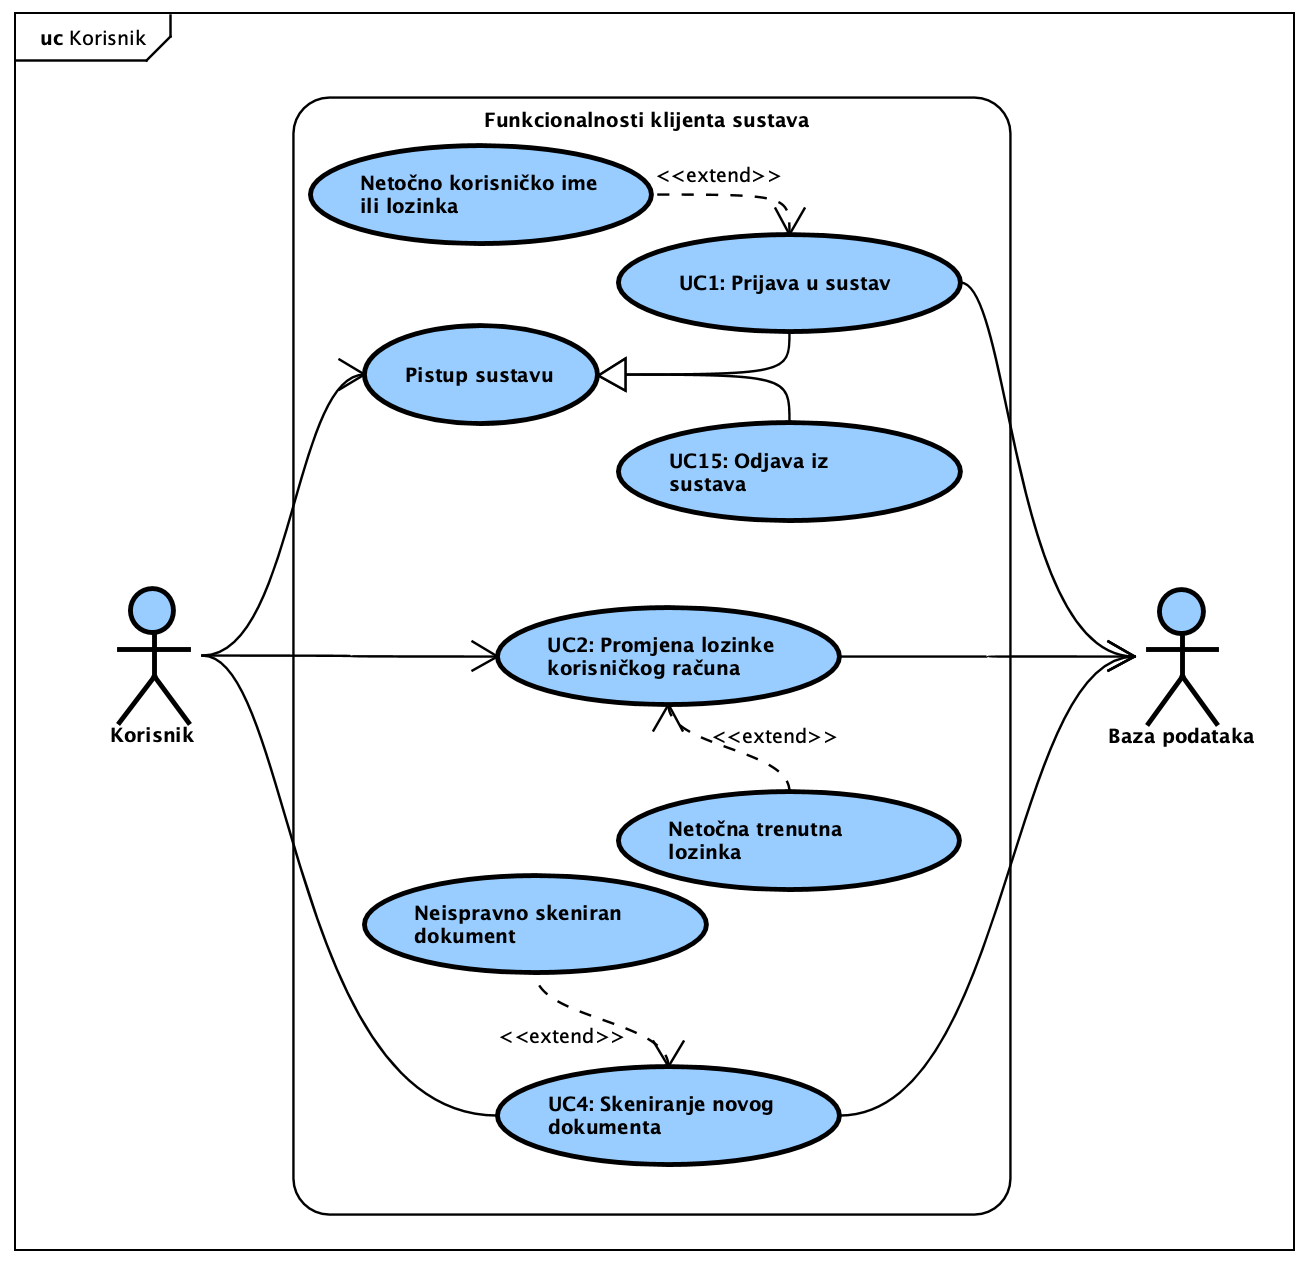
\includegraphics[width=\textwidth]{slike/UseCase_Korisnik.png} %veličina u odnosu na širinu linije
						\caption{Primjer slike s potpisom 2}
						\label{fig:usecase_korisnik} %label mora biti drugaciji za svaku sliku
					\end{figure}
					\textit{Dijagram obrasca uporabe, funkcionalnost korisnika}

					\begin{figure}[H]
						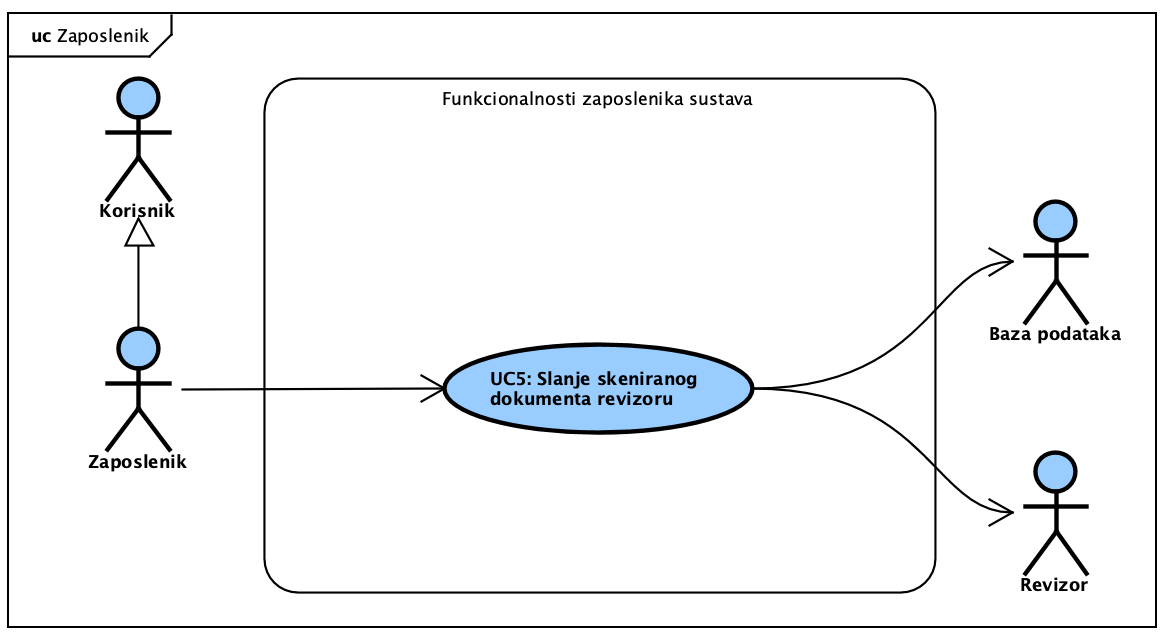
\includegraphics[width=\textwidth]{slike/UseCase_Zaposlenik.png}
						\caption{Primjer slike s potpisom 2}
						\label{fig:usecase_zaposlenik}
					\end{figure}
					\textit{Dijagram obrasca uporabe, funkcionalnost zaposlenika}

					\begin{figure}[H]
						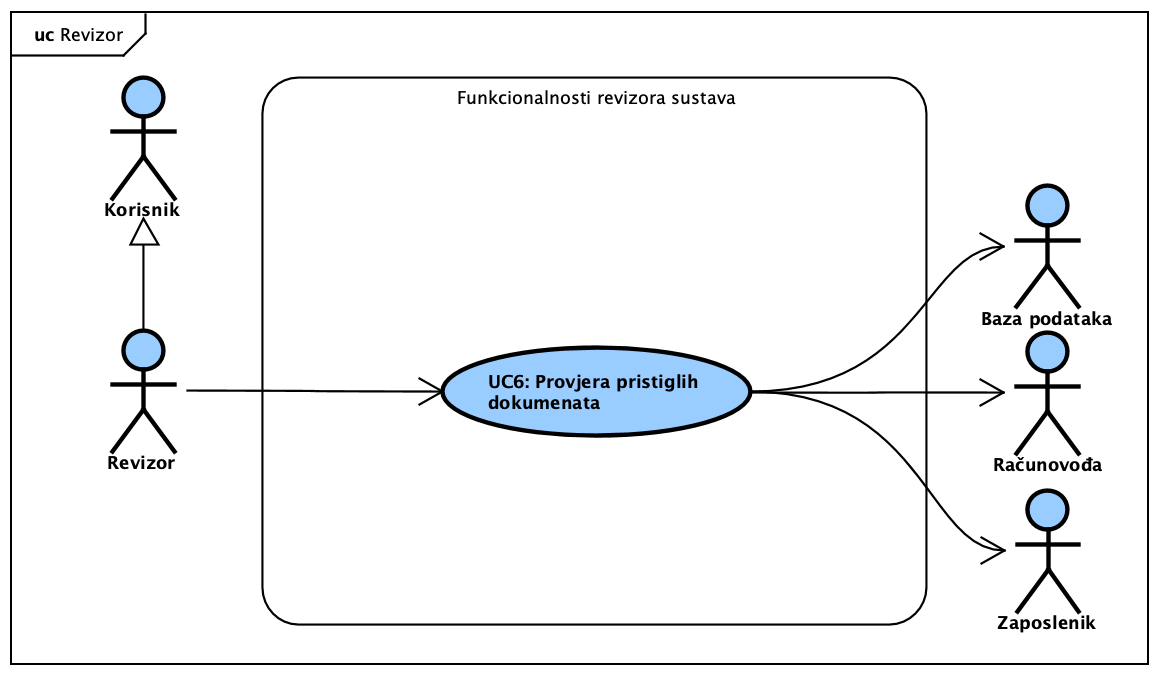
\includegraphics[width=\textwidth]{slike/UseCase_Revizor.png}
						\caption{Primjer slike s potpisom 2}
						\label{fig:usecase_revizor}
					\end{figure}
					\textit{Dijagram obrasca uporabe, funkcionalnost revizora}

					\begin{figure}[H]
						\includegraphics[width=\textwidth]{slike/UseCase_Racudovoda.png}
						\caption{Primjer slike s potpisom 2}
						\label{fig:usecase_racunovoda}
					\end{figure}
					\textit{Dijagram obrasca uporabe, funkcionalnost računovođe}

					\begin{figure}[H]
						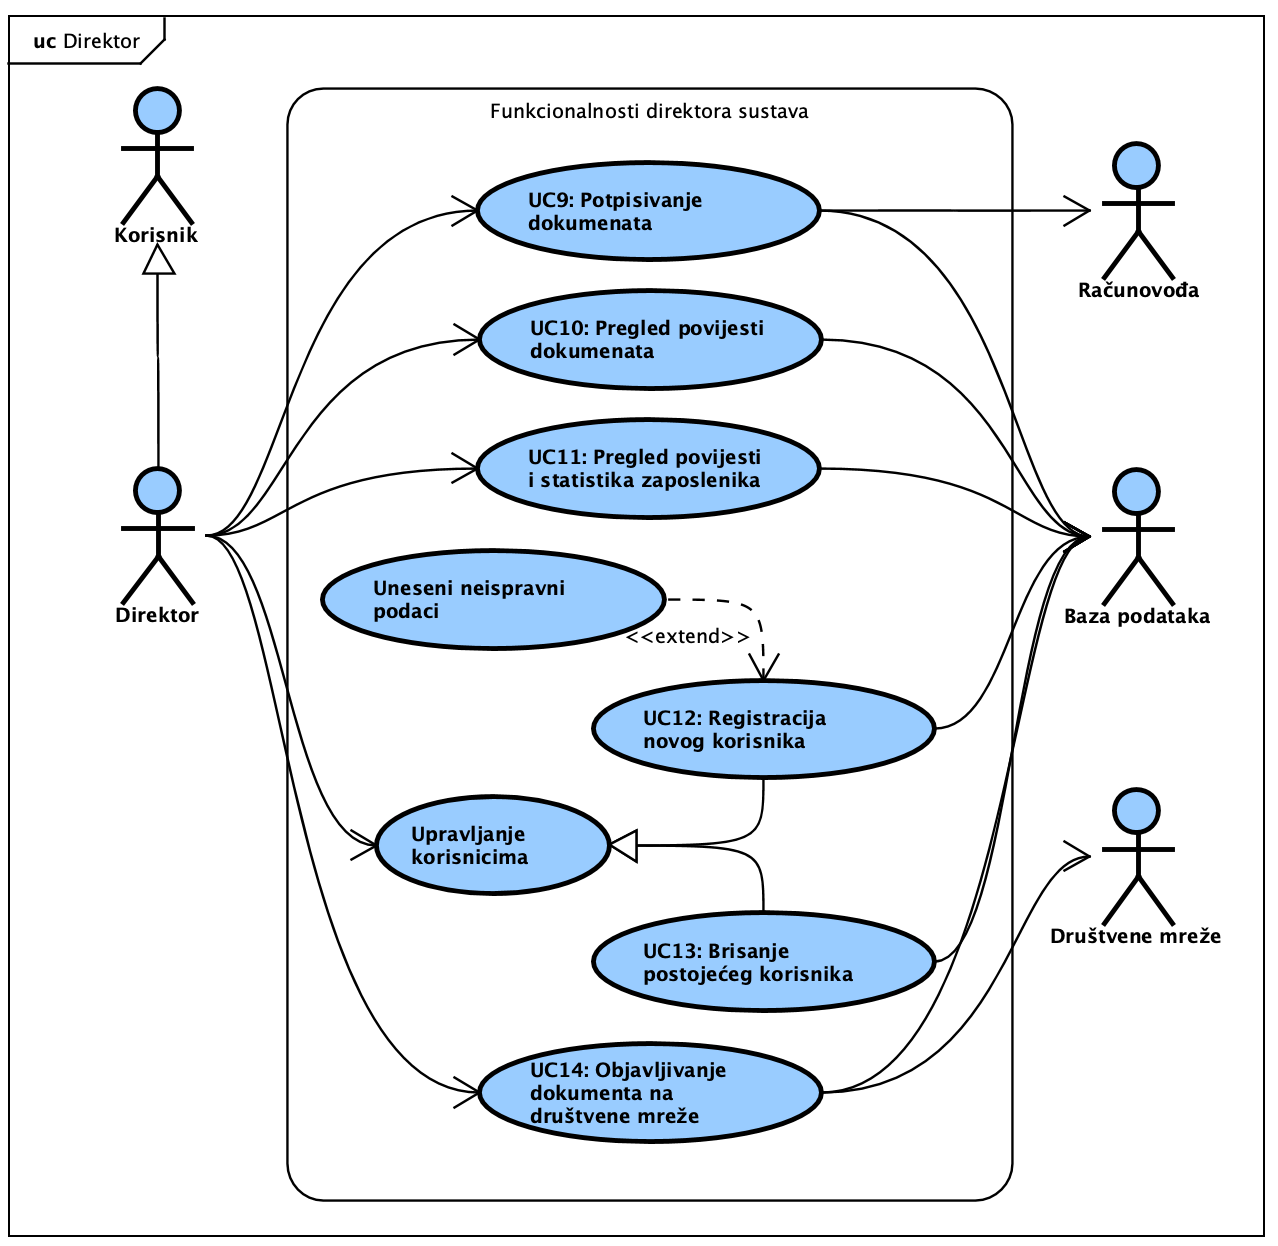
\includegraphics[width=\textwidth]{slike/UseCase_Direktor.png}
						\caption{Primjer slike s potpisom 2}
						\label{fig:usecase_direktor}
					\end{figure}
					\textit{Dijagram obrasca uporabe, funkcionalnost direktora}
				\eject{}
				
			\subsection{Sekvencijski dijagrami}
				
				\textbf{\textit{dio 1. revizije}}\\
				
				\textit{Nacrtati sekvencijske dijagrame koji modeliraju najvažnije dijelove sustava (max. 4 dijagrama). Ukoliko postoji nedoumica oko odabira, razjasniti s asistentom. Uz svaki dijagram napisati detaljni opis dijagrama.}

				\begin{figure}[H]
						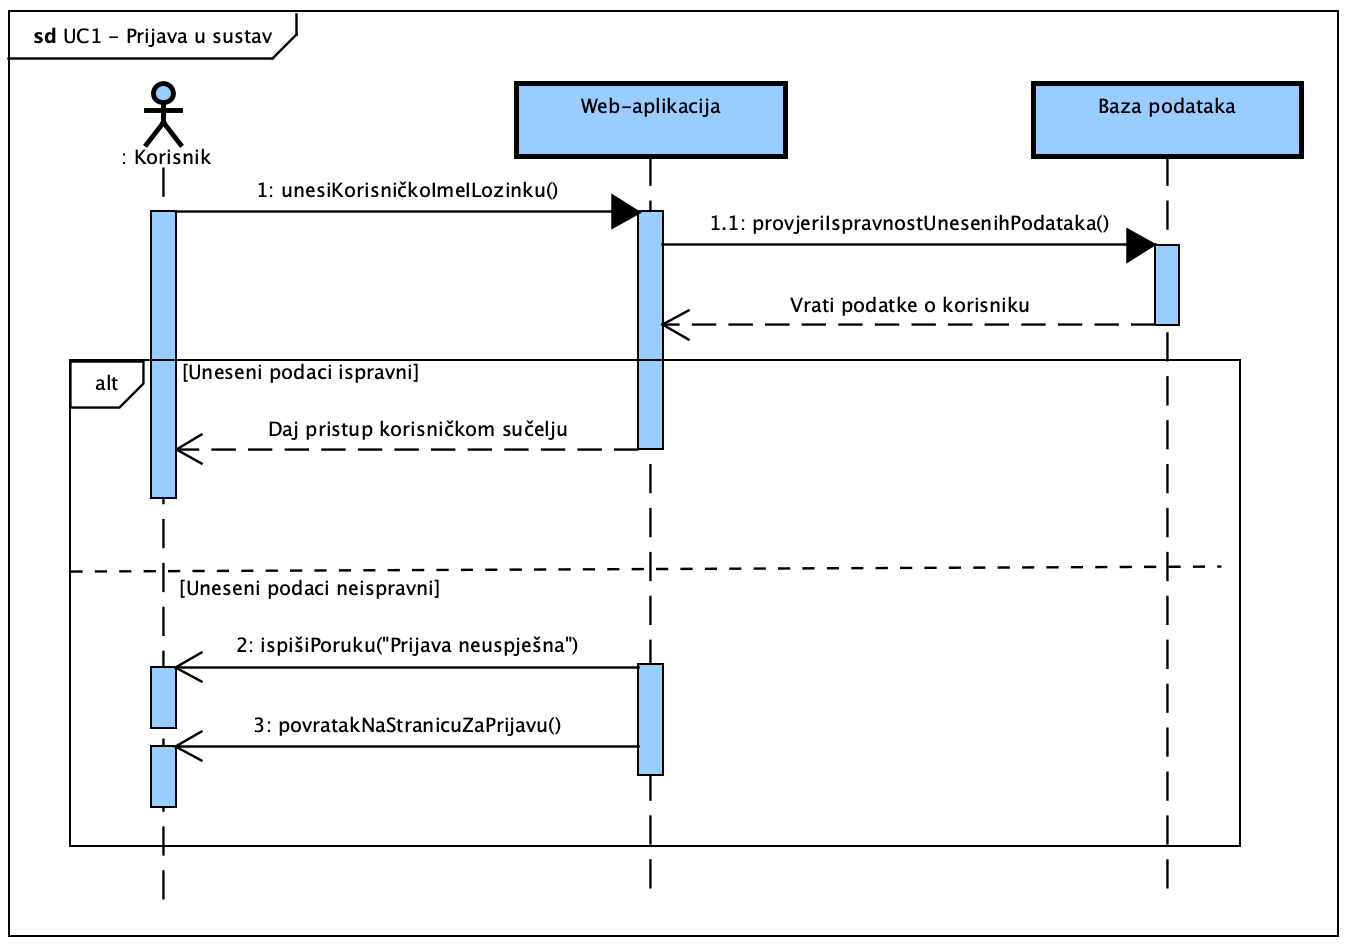
\includegraphics[width=\textwidth]{slike/Sequence_UC01.png}
						\caption{Primjer slike s potpisom 2}
						\label{fig:sequence_UC01}
					\end{figure}
					\textit{Dijagram obrasca uporabe, funkcionalnost zaposlenika}

					\begin{figure}[H]
						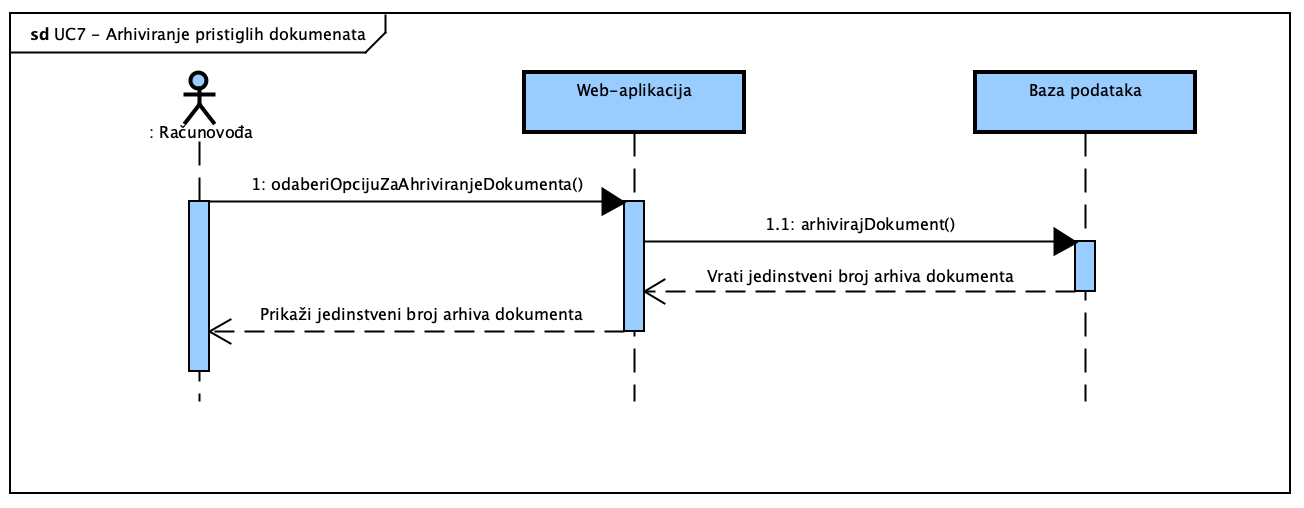
\includegraphics[width=\textwidth]{slike/Sequence_UC07.png}
						\caption{Primjer slike s potpisom 2}
						\label{fig:sequence_UC07}
					\end{figure}
					\textit{Dijagram obrasca uporabe, funkcionalnost revizora}

					\begin{figure}[H]
						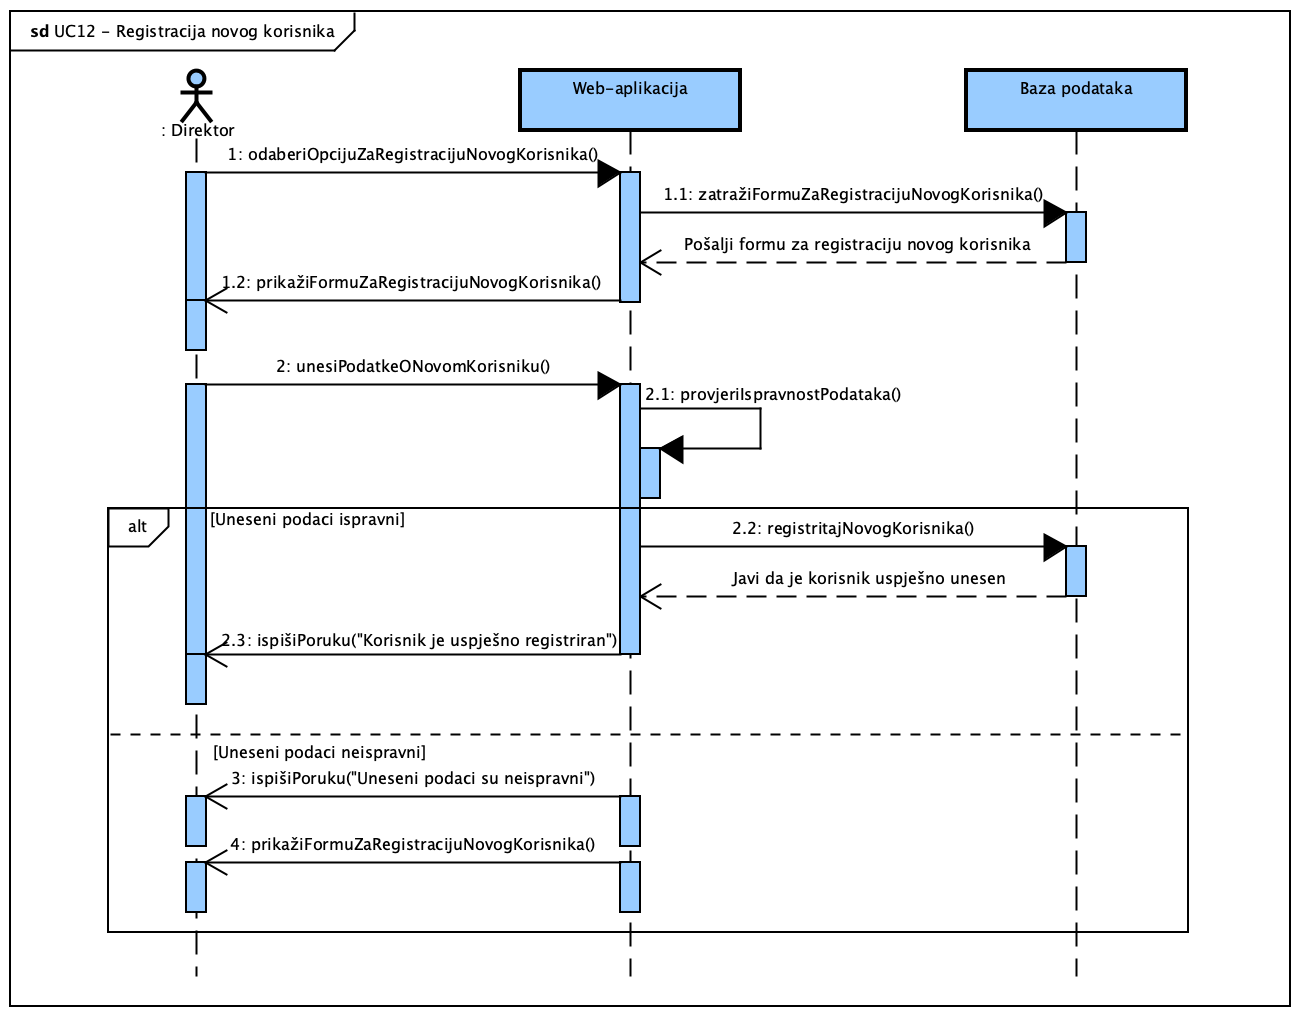
\includegraphics[width=\textwidth]{slike/Sequence_UC12.png}
						\caption{Primjer slike s potpisom 2}
						\label{fig:sequence_UC12}
					\end{figure}
					\textit{Dijagram obrasca uporabe, funkcionalnost računovođe}

					\begin{figure}[H]
						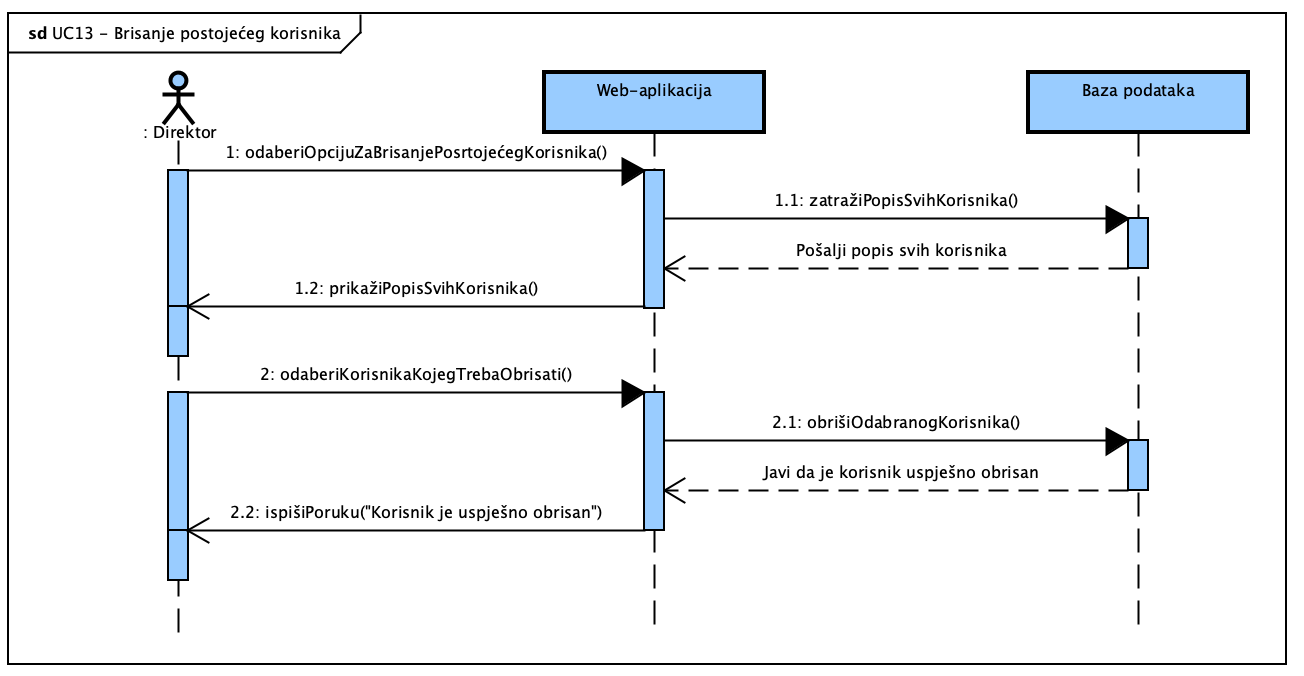
\includegraphics[width=\textwidth]{slike/Sequence_UC13.png}
						\caption{Primjer slike s potpisom 2}
						\label{fig:sequence_UC13}
					\end{figure}
					\textit{Dijagram obrasca uporabe, funkcionalnost direktora}
			\eject{}
	
		\section{Ostali zahtjevi}
		
			\textbf{\textit{dio 1. revizije}}\\
		 
			\textit{Nefunkcionalni zahtjevi i zahtjevi domene primjene dopunjuju funkcionalne zahtjeve. Oni opisuju \textbf{kako se sustav treba ponašati} i koja \textbf{ograničenja} treba poštivati (performanse, korisničko iskustvo, pouzdanost, standardi kvalitete, sigurnost...). Primjeri takvih zahtjeva u Vašem projektu mogu biti: podržani jezici korisničkog sučelja, vrijeme odziva, najveći mogući podržani broj korisnika, podržane web/mobilne platforme, razina zaštite (protokoli komunikacije, kriptiranje...)... Svaki takav zahtjev potrebno je navesti u jednoj ili dvije rečenice.}
			 
			 
			 
	